% ----------------------------------------------------------------------
%j
% TODO
%
% - spelling of ocropy, OCRopus, OCRopy
%
% ----------------------------------------------------------------------


\documentclass[conference]{IEEEtran}
\IEEEoverridecommandlockouts
\usepackage{cite}
\usepackage{amsmath,amssymb,amsfonts}
\usepackage{algorithmic}
\usepackage{graphicx}
\usepackage{rotating}
\usepackage{cleveref}
\usepackage{hyperref}
\usepackage[utf8]{inputenc}
\usepackage{textcomp}
\usepackage{xcolor}
\usepackage{multirow}
\begin{document}

\title{
okralact - foundations of a turn-key multi-engine Open Source OCR training infrastructure \\
\thanks{This work was partially supported by the Deutsche Forschungsgemeinschaft (DFG) - Project number 274863866}
}

\author{%
\IEEEauthorblockN{1\textsuperscript{st} Konstantin Baierer}
\IEEEauthorblockA{\textit{Berlin State Library} \\
konstantin.baierer@sbb.spk-berlin.de}
\and
\IEEEauthorblockN{2\textsuperscript{nd} Rui Dong}
\IEEEauthorblockA{\textit{Institut für Informatik} \\
\textit{Leipzig University}\\
dongrui@ccs.neu.edu}
\and
\IEEEauthorblockN{3\textsuperscript{rd} Clemens Neudecker}
\IEEEauthorblockA{\textit{Berlin State Library} \\
clemens.neudecker@sbb.spk-berlin.de}
}

\maketitle

% CN: Here is the call for papers: https://www.primaresearch.org/hip2019/callForPapers. For the purposes of HIP, it is important to stress the context of _historical_ documents. We can (and should, I will write sth) introduce the "problem" of historical document processing first like: a) what are the challenges of historical documents, why do we require more tailored solutions b) the possibilities of NNs and training, thus being able to train models for historical documents that can outperform off-the-shelf general OCR classifiers c) the lack of an ecosystem for Open Source OCR model generation due to (why?) i) bad usability/docs toolchain for training and their diversity and ii) lack of ground truth/standardization...you know this much better than me. This is the introduction. Then we proceed with a short discussion of Open OCR, and what the pros/cons of the selected algorithms are and why it is beneficial to be able to train all of them from one "system" - here we can e.g. argue for better evaluation/testing/replicability. Now the main part comes with the description of okralact... To close, it is important to provide a clear perspective again as to how this work will contribute to solving the challenges of historic documents from the introduction. 

\begin{abstract}

Optical character recognition (OCR) of historical documents has been much more
difficult than OCR of modern texts due to the idiosyncrasies and wide
variability of font, layout, language, orthography of printed texts before ca.
1850. Most OCR engines are optimized towards supporting the widest possible set
of modern text ("OmniFont OCR") with little or no facilities for the user to
adapt the engine. With the technologies around OCR embracing Deep Learning with
neural networks (NN), there have been various efforts to develop Free Software
OCR engines that can be adapted to different types of documents by training
specific models based on manually labeled ground truth (GT). What these
engines offer in terms of implementation finesse they lack in interoperability
and standardization. In this paper, we present okralact, a set of specifications
and a prototypical implementation of an engine-agnostic framework for training
Open Source OCR engines like tesseract, ocropus, kraken or calamari. We briefly
compare these engines, describe the specifications and software we have been
developing and outline the challenges in and our plans to contribute to
a more accessible and interoperable Open Source OCR ecosystem.

\end{abstract}

\begin{IEEEkeywords}
OCR, ocropus, kraken, calamari, tesseract
\end{IEEEkeywords}

\section*{Introduction}


The rise of deep learning in the last decade has been a game-changer for image
processing, text recognition and layout analysis, the key parts of optical
character recognition (OCR) workflows. The text recognition technology in
particular has seen a paradigm-shift, away from a combination of character
% Since training from GT is so essential for the process, all NN-based OCR engines
% offer tools to train new models. However the usability of these training tools
% varies wildly. Different engines have different assumptions n the kind of input
% data they expect, t thehe kind of haware they are run on and employ slightly different
% terminology. The tained models are engine-specific, sometime even to a specific
% version of an engine and in most cases, it is very difficult to assess what kind
% of data a model was trained on after the fact.gmentation and pattern-based detection, towards segmentation-free recognition
based on trained neural networks (NN).
%Any NN-based approach involves two steps: Training a model based on manually annotated ground truth (GT) and applying this model to data, in the case of OCR to recognize the text in images.

Most of the state-of-the-art OCR engines apply a hybrid recurrent convolutional neural network combined with a connectionist temporal classification (CTC) \cite{graves2006connectionist} layer as the OCR model. Deep convolutional neural networks (CNN) \cite{krizhevsky2012imagenet} are added as the bottom layers to extract hierarchical location-invariant features from the raw images \cite{wick2018improving}. Long shent neural networks, which are effective in capturing the dependencies in temporal sequences, are then added on top of the CNN layers to extract sequential image representations. The CTC layer allows the text recognition model to be trained on pairs of images and ground truth text without explicitly aligning between them. It both saves the efforts of segmenting the images into characters and avoids the possible errors introduced in this process. 

%Any NN-based approach involves two steps: Training a model based on manually annotated ground truth (GT) and applying this model to data, in the case of OCR to recognize the text in images.
However, these NN-based OCR engines vary wildly in their designing assumptions, e.g., the format of the input data, the hardware requirements, as well as the set of adjustable parameters for building and training the model. For example, some engines could only be run on CPU devices while the others could utilize the computation power of GPU devices. Some of them allow users to build their own neural networks while others have a fixed model structure. The trained models are engine-specific, sometimes even to a specific version of an engine and in most cases, it is very difficult to assess what kind of data a model was trained on after the fact.

% 

To overcome these obstacles to adoption, we propose \textit{okralact}, a flexible set of specifications
and a software prototype to harmonize the input data, parameterization and provenance
tracking of different engines. 

\section*{Open Source OCR}

There have been various Free Software projects that implement NN technologies
for OCR. In our work we focus on the four most prominent projects: tesseract, ocropus,
kraken and calamari.\footnote{All of the above are released with the Apache 2.0 license.}

\begin{table}[b]
\begin{tabular}{llll}
\hline
Engine    & Main Developer     & Stack                      & Development \\ \hline
OCRopus   & Tom Breuel         & Python                     & stale       \\
kraken    & Benjamin Kiessling & Python, Torch              & active      \\
Calamari  & Christoph Wick     & Python, Tensorflow         & active      \\
tesseract & Ray Smith          & C++                        & active
\end{tabular}
\caption{Basic properties of Open Source OCR engines}
\label{tab:basic}
\end{table}

\begin{table}[b]
\begin{tabular}{lllll}
\hline
Engine    & Contributors & First Release & GitHub Stars & SLOC \\ \hline
OCRopus   & 28           & 2010          & 2557         & 4996 \\
kraken    & 10           & 2015          & 146          & 4065 \\
Calamari  & 7            & 2018          & 299          & 6116 \\
tesseract & 102          & 1985          & 27135        & 143251 \\

\end{tabular}
\caption{Software metrics of selected Open Source OCR engines as of 2019-05-22}
\label{tab:stats}
\end{table}

\subsection*{OCRopus}

The brainchild of Thomas Breuel and first released in 2007, OCRopus \cite{breuel} was
initially based on tesseract. With the release of the Python implementation ocropy in
2010, OCRopus revolutionized OCR by employing Long-Short-Term-Memory (LSTM) and
bundling a set of rudimentary but usable command line tools to not only train and
apply models but also preprocess images (binarization, deskewing, layout analysis),
evaluate recognition results and a basic user interface to produce GT data. Breuel
has since moved on to create clstm, a better performing LSTM implementation 
\cite{DBLP:conf/icdar/Breuel17}, and ocropy2, a rewrite of OCRopus based on CUDA and
the PyTorch Deep Learning framework \cite{DBLP:conf/icdar/Breuel17} but neither
has reached the same traction in the Free Software community as the original Python version.

% CN: did the clstm part in ocropy introduce the NN? How can/should we refer to the current work from Tom, e.g. the PyTorch implementation? Furthermore, to satisfy the "state-of-the-art" we should say a few words about those who already successfully trained and redistributed models for historical documents. I can think of Uwe Springmann, Jesper Zedlitz, ?
% kba: No, clstm was the reimplementation of the LSTM from ocropy in C++. At this point it's effectively dead and clstm-trained models never gained traction beyond kraken < 1.0.
% kba: Ocropy2 ist alpha, hat sich seit langem nichts getan <del>gibt keine Veroeffentlichung dazu</del>.
% kba: About trianedtrained models: Bruce Roberts polytonic greek models come to mind, also https://github.com/tmbdev/ocropy/wiki/Models. Plus th

\subsection*{tesseract}

tesseract \cite{4376991} was the first Free Software OCR engine and remains one of
the oldest OCR engines still in development. Consistently helmed by Ray Smith,
tesseract has gone through various iterations and partial rewrites and changing
ownership. Open Source since 2005 and sponsored by Google since 2006, tesseract
is the most well-known and most widely used Open Source OCR engine
(c.f. Table \ref{tab:stats}).

While earlier versions of tesseract did contain training facilities that
were used in the context of OCR of historical documents, e.g. in the eMOP and
IMPACT projects, these had severe limitations and required cumbersome
character-based training with little positive effect on OCR accuracy
for historical documents.\cite{doi:10.1093/llc/fqv062}

With the release of version 4.0.0 in 2018, tesseract introduced a trainable
engine based on LSTM NN. While still a very involved, multi-step process, the
improved accuracy and fine-tuning to specific corpora outweighs the
effort. There have been efforts to streamline the training process, e.g. ocrd-train\footnote{\url{https://github.com/OCR-D/ocrd-train}.}.

% CN: Also here we can say sth about training tesseract. There is e.g. eMOP \cite{doi:10.1093/llc/fqv062} where we failed training tesseract 3 successfully for historic documents. Obviously we should mention ocrd-train here too.

\subsection*{kraken}

kraken \cite{DBLP:journals/corr/RomanovMSK17} was started as a fork of ocropy by Benjamin Kiessling in 2015 to rectify a number of issues while preserving (mostly) functional equivalence. While retaining many of the algorithms around OCR, the actual recognition engine has been based on the Torch machine learning framework since version 2.0 and can not reasonably be considered a fork of ocropy anymore.
% CN: As far as I am aware, most models for kraken are either from Ben himself or were produced via the Open Islamic Texts Initiative project, https://openiti.github.io/. 

\subsection*{calamari}

Christoph Wick has been developing the Calamari \cite{DBLP:journals/corr/abs-1807-02004}
OCR engine since 2018, based on the codebases ocropy and kraken but backed by the
TensorFlow machine learning framework.

\subsection*{Feature comparison}

% The goal of \textit{okralact} is to wrap all the engines into a common

Different OCR engines display different design features in terms of the technical details of implementation and the interfaces provided to the users. 

\subsubsection*{Implementation}

As shown in Table \ref{tab:basic}, tsseract is implemented via C++ while the other three engines are all implemented via Python.  Tesseract and OCRopus implements the neural networks as well as the inference from stratch without utilizing any existing deep learning libraries. Kraken uses PyTorch as its backend deep learning engines. Calamari provides the option of backend to the users, but currently it only supports Tensorflow.

%\subsubsection*{Library Dependencies}
\subsubsection*{Hardware Requirement}

Both Kraken and Calamari supports GPU training, which has much higher computation speed than training on CPU devices. 

\subsubsection*{Model Parameters}

Different OCR engines provides different levels of freedom for the users to    
design their own neural network structures. OCRopy does not support CNN to     
extract features from raw images. The raw image features are directly feed into
the LSTM layers. It only allows users to choose whether to use bidirectional or
unidirectional LSTM layer and the size of hidden states. The number of LSTM    
layers are fixed. Tesseract, kraken and Calamari provide more modeling options
to the users. They allow the users to add arbitrary number of CNN layers,
pooling layers, dropout layers and LSTM layers. User could choose activation
function from $sigmoid$, $tanh$, $relu$, $linear$ and $softmax$ for CNN layers
in tesseract and kraken but not in Calamari. All three engines supports user
specified  Tesseract and Kraken also support user specified stride size of
maxpooling in addition to the kernel size.

\begin{table}[bt]
\begin{tabular}{llllll}
\hline
Layers   &Parameters & OCRopus     & kraken                      & Calamari & tesseract\\ \hline
% CNN Layer& & NA & Yes & Yes & Yes  \\
\multirow{ 3}{*}{CNN} & kernel size & \multirow{ 3}{*}{NA} & Y & Y & Y  \\
& activation &  & Y & N & Y \\
& output size & & Y & Y &  Y\\\hline
\multirow{2}{*}{Pooling} &kernel size & \multirow{2}{*}{NA} &  Y & Y & Y \\
& stride size &  & Y & N & Y \\\hline
\multirow{2}{*}{Dropout} &probability & \multirow{2}{*}{NA} &  Y & Y & Y\\
&dimension &  & Y & N & Y \\\hline
\multirow{2}{*}{RNN} & output size & Y &  Y & Y & Y\\
& direction & N & Y & N & Y \\
& dynamic cell & lstm & lstm/gru & lstm & lstm/gru\\
& time axis& N & Y & Y & N \\\hline
Output & output size& N & Y & Y & N \\\hline
\end{tabular}
\caption{Model Design Options for Open Source OCR engines.}
\label{tab:model_param1}
\end{table}
\subsubsection*{Training Parameters}

\begin{table}[bt]
\begin{tabular}{llllll}
\hline
Parameters & & OCRopus     & kraken                      & Calamari & tesseract\\ \hline
% CNN Layer& & NA & Yes & Yes & Yes  \\
\multirow{2}{*}{Learning Rate}& overall & N & Y & Y & Y\\ 
&layer & N & N  & N & Y \\
\hline
Optimizer &  &  N & Y & N & Y \\\hline
Early Stop & & N & Y & Y & Y \\\hline
%& condition & & performance not & performance continuously & error rate \\
%& & & significantly improving & getting worse&  small enough\\ \hline
\end{tabular}
\caption{Training Options for Open Source OCR engines.}
\label{tab:training_options}
\end{table}
\subsubsection*{Fine Tuning}
\section*{okralact}

\subsection*{Specifications}

% * OCRD-ZIP GT format (shortly)
% * JSON schema for parameters / common API
% * https://github.com/OCR-D/spec/pull/105/files
%     * Drop the line GT part
%     * Clean up evaluation

\subsection*{Prototype}     
As shown in Figure \ref{fig:framework}, \textit{okralact} is a client/server architecture application. The interactions between the client nodes and the server are implemented via Flask, a lightweight web server gateway `interface (WSGI) web application framework. Users could upload the training or evaluation dataset and configuration files specifying the OCR engine and the parameters from the client end. The user could also submit a request of training an OCR model with the selected dataset and configuration file to the server. After the job is submitted, the user could check job status. After a model is trained, the user could download the model to client machine. The user could also submit an evaluation request with a selected evaluation dataset and a selected model.

All the jobs submitted to the server are handled by task queues. Redis Queue is utilized as the backend on the server to process job requests sent from the client end. It is a Python task queue built on top of Redis that executes work outside an HTTP request-response cycle. It would put job requests into the queue of a given worker, which serves in first-in-first-out order. When a job gets to run, it would call the common API for different OCR engines to interpret the configuration files into the training command for the specified OCR engine. 

\begin{figure*}[ht!]
        \begin{center}
     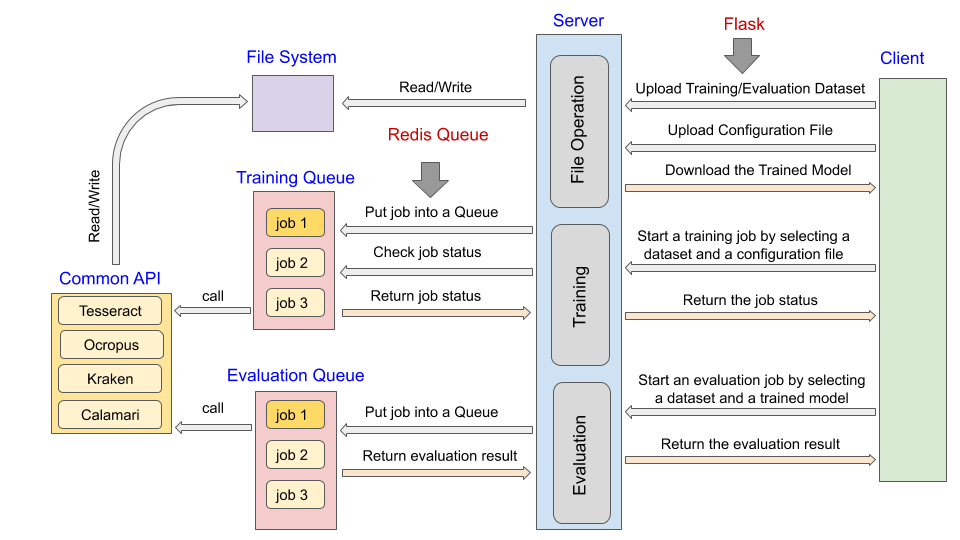
\includegraphics[width=0.8\linewidth]{Figures/Framework.png}
        \end{center}
        \caption{\small{Framework of the okralact system.}}
\label{fig:framework}
\end{figure*}

\section*{Challenges and Future Work}

% * Adapt diagram \url{https://docs.google.com/presentation/d/1jyV7pWGkIgtIrc9uJ5jbUwNthOk0JSUgT_tA2QudwkA/edit#slide=id.p}
%* Describe HTTP API
%   * Draft a `/evaluation` endpoint taking evaluation config, model, groundTruth and %returning measures like CER, WER ...

\section*{Challenges and Future Work}

% Expanded Common API by engine developers cooperating

% More flexible choice of input data (multiple works, individual lines from individual pages etc.)

% Cleanly defined evaluation measures necessary (no more ISRI or character-counting CER)

%\section*{References}

% Please number citations consecutively within brackets \cite{b1}. The 
% sentence punctuation follows the bracket \cite{b2}. Refer simply to the reference 
% number, as in \cite{IEEEexample:bluebookbook} ---do not use ``Ref. \cite{b3}'' or ``reference \cite{b3}'' except at 
% the beginning of a sentence: ``Reference \cite{b3} was the first $\ldots$''
% 
% Number footnotes separately in superscripts. Place the actual footnote at 
% the bottom of the column in which it was cited. Do not put footnotes in the 
% abstract or reference list. Use letters for table footnotes.
% 
% Unless there are six authors or more give all authors' names; do not use 
% ``et al.''. Papers that have not been published, even if they have been 
% submitted for publication, should be cited as ``unpublished'' \cite{b4}. Papers 
% that have been accepted for publication should be cited as ``in press'' \cite{b5}. 
% Capitalize only the first word in a paper title, except for proper nouns and 
% element symbols.
% 
% For papers published in translation journals, please give the English 
% citation first, followed by the original foreign-language citation \cite{b6}.

\bibliographystyle{IEEEtran}
\bibliography{bibliography}

\end{document}
